\documentclass{article}
\usepackage[utf8]{inputenc}
\usepackage{hyperref}

\author{Meng Lu, Joaquin Cavieres, Paula Moraga }
\date{September 2020}
\usepackage{amsmath}
\usepackage{natbib}
\usepackage{graphicx}
\usepackage{listings} 
\lstset{language=R,
    breaklines=true,
    basicstyle=\small\ttfamily,
    stringstyle=\color{DarkGreen},
    otherkeywords={0,1,2,3,4,5,6,7,8,9},
    morekeywords={TRUE,FALSE},
    deletekeywords={data,frame,length,as,character}
}
\usepackage{cleveref}
\usepackage{amsfonts}


\title{A comparison of INLA and machine learning-based methods in $NO_2$ modelling: prediction accuracy, uncertainty quantification, and model interpretability }
\begin{document}

\maketitle
\begin{abstract} 
Statistical spatial prediction methods are abundant and have been applied to NO2 mapping, however, current studies comparing between various statistical models focus on prediction accuracy and may not comprehensively advise optimal models. In this study, we dive into a  systematical comparison process considering prediction accuracy, uncertainty quantification, and model interpretability across spatial and non-spatial, algorithmic and data models. Multiple cross-validation methods are used to assess the prediction accuracy in different perspectives. Moreover, we evaluated stack learning methods with and without modeling spatial variations. We implemented our study using national ground station measurements of NO$_2$ in Germany and Netherlands of the year 2017, predicting NO$_2$ to 100 m resolution grid.   
%The probability distributions are calculated for latent Gaussian models and Random Forest models. The findings are extensible to boosting ensemble-tree methods. 
\end{abstract}

\section{Introduction}
NO$_2$ is a highly local, traffic-related air pollutant and negatively affect our health. High spatial resolution mapping NO$_2$ is required for providing scientific recommendations to police makers, as well as for studying the health impact and for risk assessment. Statistical methods for NO$_2$ mapping have attracted a lot of attentions with the burgeoning machine learning methods and availability of ground monitoring station networks, atmospheric satellite products, and geospatial predictors. Regularised linear regression models such as Lasso and Ridge regressions \citep{James2013introduction}, kernel methods such as support vector machine \citep{svm1999least}, ensemble tree-based statistical learning methods such as random forest \citep{breiman2001random} and boosting \citep{chen2016xgboost} are popular methods that have surged in air pollution mapping.
Most recent studies also attempt to integrate machine learning and geostatistical methods. \cite{liu2020integrate} applied krigging to the residuals from a random forest model.

Several studies compared between machine learning models and machine learning and linear regression methods \cite{chen2019comparison,kerckhoffs2019performance,luglobal,REN2020105827,machinereview} or kriging with a linear regression model. But we have not yet seen studies compare between gaussian process and machine learning models. Importantly, most studies compare only the cross-validation accuracy of the prediction mean, ignoring the prediction distributions for uncertainty quantification. Also not discussed is partition of the errors from modeling. For example, are prediction errors caused by missing co-variants,  voilating the assumptions of data distribution, non-linearity, or inconsistent distributions between training and validation sets? Moreover, the accuracy assessment in 
most studies are based on k-fold splitting \citep{kerckhoffs2019performance,larkin2017global,REN2020105827}
or bootstrapping \citep{luglobal} of ground station measurements for training and validation, which do not provide an error indication of the spatial areas where ground stations are not present for validation. Consequently, current model comparison studies may be one-sided. 

Studies apply machine learning methods commonly have a high predictive power, which may be used to improve the estimation of the mean function in a Gaussian process regression.  

In this study, our objectives are to comprehensively comparing machine learning models and GLM, in terms of their prediction accuracy, uncertainty quantification, and model interpretability. In addiction, we attempt to harness machine learning methods for a more accurate estimation of the mean function in GLM using stacked ensemble generalisation methods proposed in \cite{stackinla}. By comparing the GLM stacked ensemble with non-spatial stacked ensemble using the same base learners we can understand the amount of spatial information that is not represented by machine learning methods.  
    %and their potential in providing information for model improvement (indicating missing co-variates).
    


%    \item Propose a framework for model comparison and spatial validation. 
    %and an optimal statistical model for high-resolution NO$_2$ mapping.
 
Three statistical learning methods, Lasso, XGBoost, and Random Forest (RF) are chosen for the comparison with the LGM and form the base learners in stacked learning. Integrated Nested Laplace Approximation (INLA) is used for LGM model implementation.  The machine learning methods are chosen for their dissimilarity: Lasso is a linear model without accounting for spatial dependency, which is modelled in a LGM as spatial random effects. RF and XGBoost are non-linear and are not affected by dependent co-variates, with the later build tree models subsequently over the residuals of previous trees and has multiple routines to penalise model over-fittng, which has been reported in various studies to obtain the highest prediction accuracy.

The second goal is achieved by embedding machine learners in a Gaussian process regression \citep{stackinla}. This method is compared with stacked modeling using  the same super-learner without modeling the spatial random effects. 

 
 
\section{Data}
We used average NO2 concentration of 2017 from ground stations in Netherlands and Germany.

\section {Methods}
 
We focus on comparing the prediction accuracy, uncertainty assessment and model interpretability between a GLM and several machine learning models. The prediction accuracy are compared for the following models.   
\begin{enumerate}
    
\item "INLA": a Bayesian hierarchical model using INLA  assuming a Gaussian prior;
\item Lasso; 
\item "RF": Random Forest; 
\item "XGB": XGBoost assuming a Gaussian loss; 
\item "XGB-gamma": XGBoost assuming a gamma loss; 
\item "RF+Lasso": RF in post-processing using Lasso \citep{hastie2009elements}; 
\item "Stacked": stacked learning of Lasso, RF, XGBoost models; 
\item INLA stacked learning of Lasso, RF, XGBoost models. 
\end{enumerate}

The uncertainty assessments are compared between INLA and two types of distributional random forest methods, namely quantile regression forest \citep{meinshausen2006quantile} and distributional forest \citep{schlosser2019distributional}. The quantile regression forest is implemented for RF+Lasso.  %Among the ML methods, only the distribution prediction and interpretability from INLA and RF are compared, as INLA is representative to Gaussian process models and RF an ensemble tree model.
%The reason we choose random forest method to represent the XGB and Lasso is due to the good prediction accuracy obtained by RF+Lasso
Model interpretation is compared between XGBoost, RF, and INLA.

We refer  Lasso and RF to excellent illustrations in classical machine books \citep{hastie2009elements,James2013introduction} and RF and XGBoost to the original papers \citep{breiman2001random,chen2016xgboost} and introduce INLA, RF+Lasso, and stacked modeling in the sections below.

\subsection{Spatial modeling}
\subsubsection{Spatial random field}
A spatial random field is a stochastic spatial process generally defined by $\{X(\boldsymbol{s}): \boldsymbol{s} \in D \subset \mathcal{R}^{d}\}$, where $\boldsymbol{s}$ is the location in the space (e.g. latitude-longitude pairs) for the spatial process $X(\boldsymbol{s})$ and $D$ is the spatial domain. A spatial random field is a Gaussian random field if $\{X(\boldsymbol{s}_{1}),...., X(\boldsymbol{s}_{n})\} \sim \mathcal{N}_{n}(\boldsymbol{0}, \boldsymbol{\Sigma})$, where $N_{n}$ is a Normal multivariate distribution for the spatial process and is completely specified by it's mean $\mu = \mathbb{E}(X(\boldsymbol{s}))$, and the covariance function $C(\boldsymbol{s}_{1}, \boldsymbol{s}_{2}) = \text{Cov}(X(\boldsymbol{s}_{1}), X(\boldsymbol{s}_{2}))$. The Gaussian random field can be stationary and isotropic, where the covariance function depend only on the distance and not direction between points, that is $C(\boldsymbol{s}_{1}, \boldsymbol{s}_{2}) = \text{Cov}(\|\boldsymbol{s}_{1} - \boldsymbol{s}_{2}\|)$ and it's dependence is commonly modeled by a Matérn function (\cite{stein2012interpolation}\cite{yuan2011models}). Since incorporating the spatial dependence directly with a large number of observations using a Gaussian random field is computationally expensive, \cite{rue2005gaussian} proposed the approximation of a Gaussian random field by a Gaussian Markov random field for a more efficient computational process of estimation. The main property of the Gaussian Markov random field is that it uses a conditional dependency structure through the precision matrix $\boldsymbol{Q}$.


\subsubsection{The SPDE (Stochastic partial differential equation) method}

To modeling data indexed in space, \cite{lindgren2011explicit} proposed a new methodology based mainly on the approximation of the Gaussian random field with the Matérn function using the Stochastic Partial Differential Equations (SPDE) as follow:

\begin{equation}\label{eqn:eq1}
(\kappa^{2} - \Delta)^{\alpha/2}(\tau(\boldsymbol{s}) x(\boldsymbol{s})) = \boldsymbol{\mathcal{W}(s)},
\end{equation}
 
where $\kappa$ is a scale parameter, $x(\boldsymbol{s})$ is a spatial random field, $\Delta$ is the Laplacian, $\alpha$ is the parameter that controls the smoothness of the realizations, $\tau$ controls the variance and $\boldsymbol{\mathcal{W}(s)}$  is a Gaussian spatial white noise process (\cite{lindgren2015bayesian}). For the above we can use a Gaussian Markov random field that approximates to a Gaussian random field without specifying an explicit covariance structure through the SPDE method. This approximation leads to a decrease in the computational burden from $\mathcal{O}(n^{3})$ to $\mathcal{O}(n^{3/2})$. 


\subsubsection{Bayesian inference}

 The \texttt{R} package \texttt{INLA} facilitates the application of the Integrated Nested Laplace Approximation (INLA) method to performs direct numerical calculation of the posterior distribution for a Bayesian hierarchical model (\cite{rue2009approximate}\cite{martino2009implementing}). If we use $\boldsymbol{x}$ as a latent Gaussian field (a Gaussian Markov random field), $\boldsymbol{\theta}$ a vector of (hyper)parameters and $\boldsymbol{y}$ a vector of observations, assuming independent observations given the vector of the spatial latent field ($\boldsymbol{x}$) and the hyperparameters ($\boldsymbol{\theta}$), the likelihood can be expressed as:

\begin{equation} \label{eqn:eq2}
p(\boldsymbol{y}\mid \boldsymbol{x},\boldsymbol{\theta}) =\prod_{i\in \mathcal{I}} p(y_i|\eta_i,\boldsymbol{\theta}),
\end{equation}

where $\eta_{i}$ is the linear predictor and $\mathcal{I}$ contains the indices for the observed values $\boldsymbol{y}$.  \\

The main idea is to approximate the posterior density for the posterior of the spatial latent field and the hyperparameters, hence, the marginal densities can be obtained:

\begin{equation} \label{eqn:eq3}
p(x_i \mid \boldsymbol{y}) = \int p(x_i \mid \boldsymbol{\theta},\boldsymbol{y})  p(\boldsymbol{\theta} \mid \boldsymbol{y}) d\boldsymbol{\theta},
\end{equation}
and
\begin{equation} \label{eqn:eq4}
p(\boldsymbol{\theta}_j|\boldsymbol{y}) = \int p(\boldsymbol{\theta} \mid \boldsymbol{y})  d\boldsymbol{\theta}_{-j}.
\end{equation}
respectively (\cite{lindgren2015bayesian}\cite{krainski2018advanced}). \\

\subsection{Model for data}

The general structure for a Bayesian hierarchical model in INLA is as follows:


\begin{align}
\boldsymbol{\theta} \hspace{2mm} \sim & \hspace{2mm} \pi(\boldsymbol{\theta}) \label{eqn:eq5}\\
\boldsymbol{x} \mid \boldsymbol{\theta} \hspace{2mm} \sim & \hspace{2mm} \mathcal{N}(\boldsymbol{0}, \boldsymbol{Q}(\boldsymbol{\theta})^{-1}) \label{eqn:eq6}\\
\eta_{i} \hspace{2mm} = & \hspace{2mm} \sum_{j}b_{ij}x_{j}\label{eqn:eq7}\\
\boldsymbol{y} \mid \boldsymbol{x}, \boldsymbol{\theta} \hspace{2mm} \sim & \hspace{2mm} \prod_{i \in \mathcal{I}}p(\boldsymbol{y} \mid \boldsymbol{\eta}, \boldsymbol{\theta}) \label{eqn:eq8},
\end{align}

where $\boldsymbol{\theta}$ is the vector of hyperparameters with $\text{log}(\tau) = \theta_{1}$ and $\text{log}(\kappa) = \theta_{2}$,  $\boldsymbol{x}$ is the spatial latent field, $\boldsymbol{\eta}$ is the linear predictor with covariates $b_{ij}$ and $\boldsymbol{y}$ is the vector of the response variable $f(\cdot \mid \boldsymbol{x}, \boldsymbol{\theta})$, commonly belonging from the exponential family of distributions. 
\vspace{0.2cm}




\subsection{Stacked learning}
Stacked learning is trained based on the cross-validation of different learners, in this case the three learners are predictions from RF, XGBoost, and Lasso models. Two super learners are compared, one is the native optimisation, and the other incorporates a gaussian process model (here INLA) to model the spatial random effects. 

\subsection{RF with Lasso in post-processing}

In this study, we also implement the RF post-processing method proposed in \cite{hastie2009elements} RF with Lasso in post-processing (called "



\section{Modeling process}

\subsection{Hyperparameter setting for XGBoost and random forest}
\label{sec:hp}

To tune XGBoost, we used grid search to optimise hyperparameters in 5-fold cross-validation basing on the minimum RMSE (Root Mean Squared Error) and additionally manual adjustment of the hyperparameters to look at the prediction patterns. The search grid for the number of iterations (nrounds) was from 200 to 3000, with a step of 200; maximum tree depth (max-depth) from 3 to 6 with a step of 1, learning rate (eta) from 0.001 to 0.1 with a step of 0.05, the penalty term gamma \citep{xgboost}  from 1 to 5 with a step of 1, the subsample is set to 0.7, L1 norm penalisation (lambda) is set to 2 and L2 norm penalisation (alpha) is set to 0.  The optimal setting for RF is min.node.size equals 5 and mtry equals 12, the number of trees is set to 1000 for random forest, which is a safe choice as the high number of trees will not negatively affect model performance. The final setting for XGB is: nround = 3000, eta = 0.007, subsample = 0.7, max-depth = 6, gamma =5, lambda =2, alpha = 0. 

RF is not sensitive to hyperparameter tuning. We used the default setting of number of variables that are randomly drawn for each tree\citep{breiman2001random}, which is the integer part of the total number of variables divided by three. The number of trees is set to 1000. 


\subsection{Variable selection for INLA} 

The INLA is used in two models:  applying to predictor variables as other methods and stacked modeling. Before applying INLA to predictor variables, we used Lasso to reduce the number of variables. The Lasso is used in contrast to ensemble tree-based methods as they are both linear models. 
Variables are selected with the L1 norm penalty that gives the model whose error is within one standard error of the minimum mean cross-validated error.

We bootstrapped data 20 times, and used variables that are selected more than 10 times by the Lasso model (with hyper-parameter optimised in \cref{sec:hp}). The frequency that the Lasso selected a certain variable is shown in \cref{lassoselect}. The INLA modeling process applies the same bootstrapped samples for training and validation. 

  \begin{table}[!htbp] \centering 
  \caption{Frequencies (number of times) of variables selected by Lasso in 20 times bootstrapping. We only show variables that are selected more than 90\% of the times (i.e. 18). These variables are considered in INLA besides road\_class\_3\_3000 as it is highly correlated with road\_class\_1\_5000.} 
  \label{lassoselect} 
\begin{tabular}{@{\extracolsep{5pt}} ccc} 
\\[-1.8ex]\hline 
\hline \\[-1.8ex] 
 & Variables & Frequency \\ 
\hline \\[-1.8ex] 
 1 & nightlight\_450 & $20$ \\ 
2 & population\_1000 & $20$ \\ 
3 & population\_3000 & $20$ \\ 
4 & road\_class\_1\_5000 & $20$ \\ 
5 & road\_class\_2\_100 & $20$ \\ 
6 & road\_class\_3\_300 & $20$ \\ 
7 & trop\_mean\_filt & $20$ \\ 
8 & road\_class\_3\_3000 & $19$ \\ 
9 & road\_class\_1\_100 & $18$ \\ 
%10 & road\_class\_3\_100 & $14$ \\ 
%11 & road\_class\_3\_5000 & $6$ \\ 
%12 & road\_class\_1\_300 & $5$ \\ 
%13 & road\_class\_1\_500 & $5$ \\ 
%14 & road\_class\_2\_1000 & $2$ \\ 
%15 & nightlight\_3150 & $1$ \\ 
%16 & road\_class\_2\_300 & $1$ \\ 
%17 & road\_class\_3\_1000 & $1$ \\ 
%18 & temperature\_2m\_7 & $1$ \\  
 
\hline \\[-1.8ex] 
\end{tabular} 
\end{table} 

\subsection{INLA model parameterisation}


\subsection {Prediction intervals}

CRPS (Continuous Ranked Probability Score) \citep{jordan2017evaluating} is used to evaluate the probability distribution predicted in INLA and RF+Lasso (representing machine learning-based methods) for uncertainty quantification. The prediction quantiles for each methods are calculated as follows. %The coverage probability is calculated as the ratio between the number of  predictions within the upper and lower quantile and the total number of predictions. 
\begin{itemize}
     
\item INLA
The prediction intervals of INLA is calculated by simulating from the response Y $\sim N(\theta, sigma^2)$.  

%inputs needed from Joaquine or Paula

\item Random Forest 
 The predictive quantiles of RF are calculated in two ways, one uses all the observations in each terminal node and over all the trees as a predicted distribution for each terminal node, known as quantile regression forest \citep{meinshausen2006quantile}. The other embeds the GAMLSS \citep{stasinopoulos2007generalized} into RF, known as distributional forests \citep{schlosser2019distributional}, which for each tree uses standard maximum likelihood to fit distributions and recursively select and split co-variates according to the instability of the gradient of the likelihood at each observation along each co-variate. 
 
\subsection{Model interpretation}
For a linear model like INLA, the best explanation model is the linear model itself but for ensembling methods it is harder to interpret the models \citep{NIPS2017_8a20a862}. We use SHAP \citep[SHapley Additive exPlanations,][]{lundberg2018explainable,NIPS2017_8a20a862}, a unified method based on additive feature-attribution, to estimate variable influence in respectively the RF and XGBoost models.   
%For a linear model like INLA, the best explanation model is the linear model itself but for ensembling methods it is harder to interpret the models \citep{NIPS2017_8a20a862}. We use SHAP \citep{NIPS2017_8a20a862} to interpret the ensemble tree models.

\subsection{Spatial validation}
Besides 20-times random bootstrapping, We also used two other spatial validation methods to comprehensively evaluate the models at different angles.

\begin{enumerate}
 %   \item Probability sampling: higher probability is given to select observations that are isolated, to test how good the model is at predicting air pollution over the whole region. This is because with random sampling we would get more points in areas where observations are clustered and may not pick any observation in areas with few observations.   
    \item Spatial blocked cv: divide the data into spatial blocks, each time use one block for validation and other blocks for training. 
    \item Validation based on customised predictors: based on predictor values, we divided the study area so that we assess the prediction accuracy for certain areas. In this study, three subareas are defined:  1) close to traffic and high population:  
    2) close to traffic and middle low population. 3) far away from traffic. High population is defined as the variable population of 1000 m buffer that is in the last quartile. Low population is defined as the variable population of 1000 m buffer is below the median. Close to road is defined as: 
    \begin{lstlisting} 
    road_class_2_100 > 0 | 
    road_class_1_100 > 0 |
    road_class_3_100 > quantile(road_class_3_100, .75)) \end{lstlisting}
    Far away from road is defined as:
  \begin{lstlisting} 
    road_class_2_100 == 0 &
    road_class_1_100 == 0 & 
    road_class_3_100 < quantile(road\_class\_3\_100, .5)
    
    \end{lstlisting}
    where "{\tt \&}" indicates "and" and "{\tt |}" indicates "or". the second variable of the function "{\tt quantile(.)}" indicates the percentage quantile of the variables. 
   
    \item Validation based on known attribute: we know the air quality station types (traffic, background, industrial) and human settlement types (urban or rural), this allows us to quantify prediction accuracy for each type of air quality stations and separating between urban and rural areas. 
\end{enumerate}

%\item XGboost
%Quantile regression is used to calculate the prediction quantiles of XGBoost, based on \cite{quantile} 

%\item Lasso

\end{itemize}
 
\section{Results}
\subsection{Prediction Accuracy}


\begin{table}[!htbp] \centering 
  \caption{Prediction accuracy matrix for different models using 20 times bootstrapped cross-validation. LA: Lasso; RF: random forest, XGB: XGBoost using the default gaussian loss; XGB-G: XGBoost using a gamma loss; RFLA: random forest with lasso for schrinkage aggregation of regression trees. INLA: Latent gaussian model using INLA, assuming a gaussian  } 
  \label{} 
\begin{tabular}{@{\extracolsep{5pt}} cccccccccc} 
\\[-1.8ex]\hline 
\hline \\[-1.8ex] 
         & LA & RF & XGB & XGB-G & RFLA & INLA& INLA-G &SE& SE-INLA\\ 
\hline \\[-1.8ex] 
RMSE & $7.54$ & $7.45$ &$7.14$ & $8.91$ & $7.23$ & $7.06$ & 9.21 &7.18 & $6.83$\\ 
IQR & $8.47$ & $7.39$ & $6.54$ & $9.21$ & $7.27$ & $7.1$ & 7.4 &7.30& $6.8$\\ 
MAE & $5.69$ & $5.51$ & $5.05$ & $6.27$ & $5.28$ & $5.3$ & 6.2  &5.31& $5.0$\\ 
 
R$^2$ & $0.65$ & $0.65$ & $0.68$ & $0.51$ & $0.67$ & $0.69$ &  0.45& 0.69& $0.71$\\ 
\hline \\[-1.8ex] 
\end{tabular} 
\end{table} 
\subsection{Distributional forest vs. quantile regression trees}

Both the distributional forest and quantile regression trees reach the coverage probability higher than 0.9, but the distributional forest predict a more realistic prediction quantile, notably, it covers four observations that are not covered by the prediction quantile predicted by the quantile regression forest. 

\begin{figure}
\centering
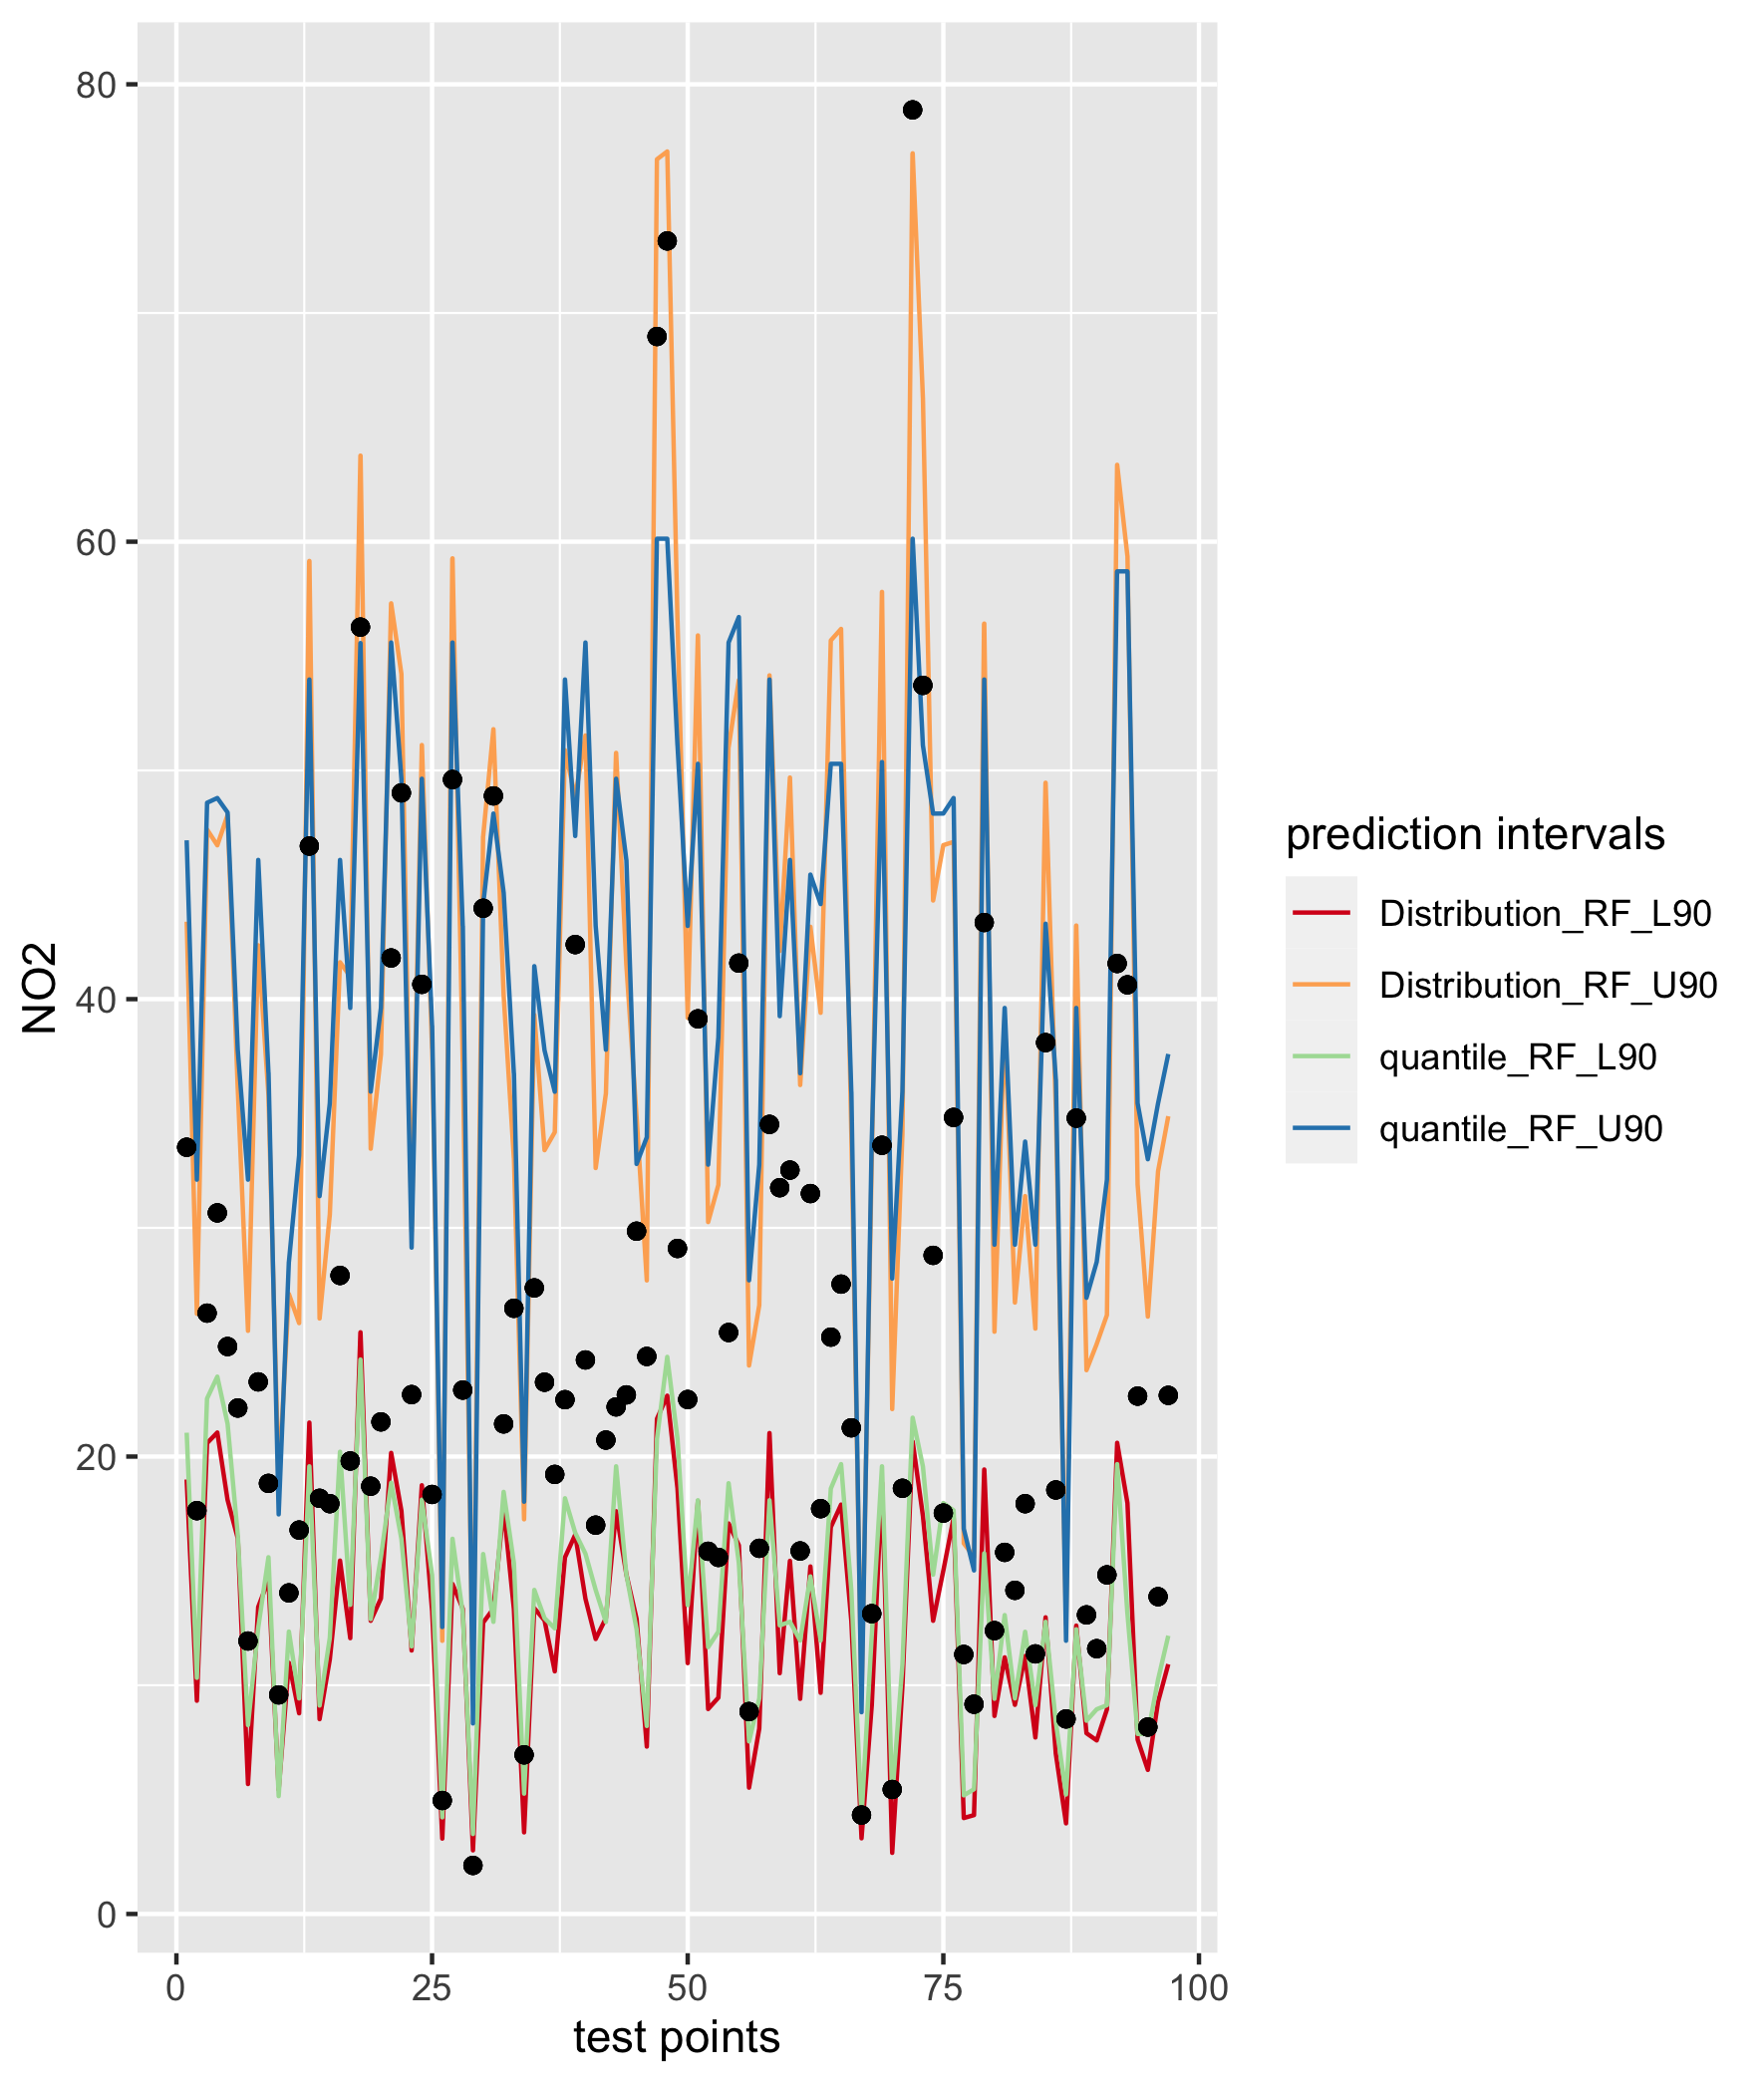
\includegraphics[scale = 0.2]{fig/dist_vs_qrf.png}
\caption{The 90\% prediction interval predicted by distributional forest and quantile regression trees. The black dots indicate observations in the test dataset.}
\label{distvsquant}
\end{figure}

\subsection{Model Interpretation} 


For a linear model like INLA, the best explanation model is the linear model itself but for ensembling methods it is harder to interpret the models \citep{NIPS2017_8a20a862}. We use SHAP \citep{NIPS2017_8a20a862} to interpret the ensemble tree models.

SHAP values are calculated separately for RF and XGBoost methods using all the data. The variables are ranked by their variable importance, which is calculated as the sum of SHAP magnitudes over all the samples. It can be observed from \cref{rfshap} and \cref{xgbshap} that the variable rankings are similar and the number of points that have positive or negative impact are similar. Both methods ranked road\_class\_2\_100 at the top. The SHAP values also indicate a realistic pattern of the sample influence. 

% do they give the same interpretation?
\begin{figure}
\centering
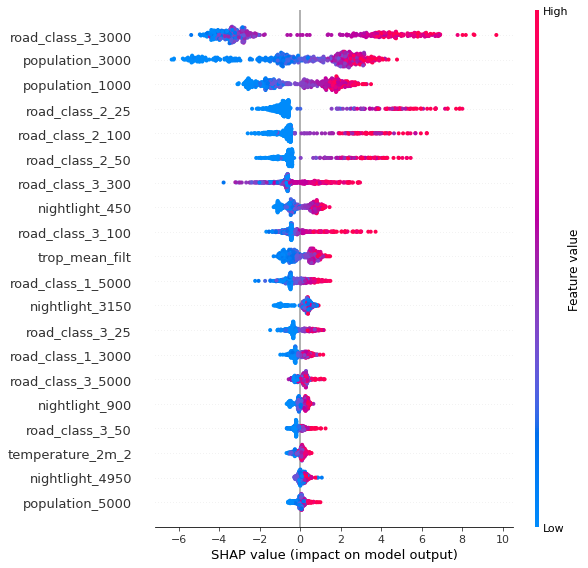
\includegraphics[scale = 0.5]{fig/rfshap.png}
\caption{Variable impact calculated by SHAP, the RF model. The horizontal location shows whether the effect of that value is associated with a higher or lower prediction. The ranking is based on the sum of SHAP magnitudes over all the samples.}
\label{rfshap}
\end{figure}

\begin{figure}
\centering
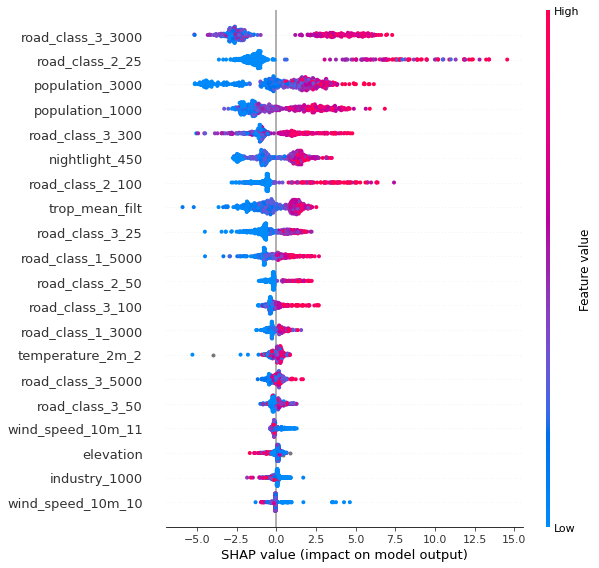
\includegraphics[scale = 0.5]{fig/xgbshap.png}
\caption{Variable impact calculated by SHAP, the XGBoost model. The horizontal location shows whether the effect of that value is associated with a higher or lower prediction. The ranking is based on the sum of SHAP magnitudes over all the samples.}
\label{xgbshap}
\end{figure}


\section{Discussion}
The advantage of INLA.


\newpage
\bibliographystyle{plain}
\bibliography{references}
\end{document}

Other: the newest boosting technique, Catboost, gives the best cross validation results, with same learning rate as xgboost and number of iterations. But it's not convenient for now to ensemble it as it is not yet in h2o. 

                    Catboost
RMSE          7.0 
RRMSE         0.3 
IQR           6.4 
rIQR          0.3 
MAE           5.0 
rMAE          0.2 
rsq           0.70 
explained\_var 0.70

with spatial cv
                    INLA 
                    
RMSE          10.0900074
RRMSE          0.3023047
IQR           11.6697717
rIQR           0.3894527
MAE            7.4846970
rMAE           0.2242679
rsq            0.3630397
explained\_var  0.4319317
 
 Lasso
RMSE	10.0900074			
RRMSE	0.3023047			
IQR	11.6697717			
rIQR	0.3894527			
MAE	7.4846970			
rMAE	0.2242679			
rsq	0.3630397			
explained\_var	0.4319317	

RF
RMSE	9.6393525			
RRMSE	0.2888581			
IQR	11.6795936			
rIQR	0.3899266			
MAE	7.2699949			
rMAE	0.2178434			
rsq	0.4176984			
explained\_var	0.4752084			
covprob90	0.9063574	

XGB 
RMSE	9.6618743			
RRMSE	0.2895155			
IQR	10.1181299			
rIQR	0.3379141			
MAE	7.0342845			
rMAE	0.2107836			
rsq	0.4140045			
explained\_var	0.4960338

Stacked INLA
RMSE           8.48140767
RRMSE          0.25475534
IQR           10.50499614
rIQR           0.35099809
MAE            6.53715007
rMAE           0.19644237
rsq            0.54917218
explained\_var  0.55811686
cor            0.75390795
covprob95      0.21804124
covprob90      0.17989691
covprob50      0.08092784


If I choose clustered points with high prob (big city?), the result is similar to random sampling, and better accuracy. 

 

If I choose scattered points with high prob (does it mean more rural points?), there is very little randomness. result is also worse. --> the reason for scattered points with high prob. is because they contain more info?
there are a lot more clustered points (as the hist. peak at small prob). so the scattered points will be selected first, that is the reason there is little randomness. 

 
\subsection{Variable importance}
   \begin{table}[!htbp] \centering 
    \caption{Variable importance ranked by XGBoost and Random Forest. The ranking is based on variable importance averaged over 20 times bootstrapping.} 
    \label{vimp} 
  \begin{tabular}{@{\extracolsep{5pt}} ccc} 
  \\[-1.8ex]\hline 
  \hline \\[-1.8ex] 
  rank & XGBoost & Random Rorest \\ 
  \hline \\[-1.8ex] 
  1 & population\_3000 & population\_3000 \\ 
  2 & road\_class\_3\_3000 & road\_class\_2\_100 \\ 
  3 & population\_1000 & road\_class\_3\_3000 \\ 
  4 & nightlight\_450 & population\_1000 \\ 
  5 & road\_class\_2\_100 & nightlight\_450 \\ 
  6 & road\_class\_3\_300 & nightlight\_3150 \\ 
  7 & road\_class\_1\_5000 & population\_5000 \\ 
  8 & nightlight\_3150 & road\_class\_3\_300 \\ 
  9 & road\_class\_3\_100 & nightlight\_900 \\ 
  10 & population\_5000 & road\_class\_3\_5000 \\ 
  11 & trop\_mean\_filt & road\_class\_2\_300 \\ 
  12 & radiation & road\_class\_3\_100 \\ 
  13 & nightlight\_900 & nightlight\_4950 \\ 
  14 & road\_class\_3\_5000 & trop\_mean\_filt \\ 
  15 & road\_class\_1\_100 & road\_class\_1\_5000 \\ 
  16 & nightlight\_4950 & industry\_5000 \\ 
  17 & temperature\_2m\_2 & road\_class\_1\_3000 \\ 
  18 & road\_class\_1\_3000 & temperature\_2m\_2 \\ 
  19 & elevation & road\_class\_2\_500 \\ 
  20 & industry\_5000 & elevation \\ 
 
  \hline \\[-1.8ex] 
  \end{tabular} 
  \end{table} 
  
  
  \begin{table}[!htbp] \centering 
  \caption{} 
  \label{} 
\begin{tabular}{@{\extracolsep{5pt}} ccccc} 
\\[-1.8ex]\hline 
\hline \\[-1.8ex] 
 & LA & RF & XGB & RFLA \\ 
\hline \\[-1.8ex] 
RMSE & $7.54$ & $7.40$ & $7.10$ & $7.24$ \\ 
RRMSE & $0.32$ & $0.32$ & $0.30$ & $0.31$ \\ 
IQR & $8.42$ & $7.22$ & $6.27$ & $7.26$ \\ 
rIQR & $0.39$ & $0.34$ & $0.29$ & $0.34$ \\ 
MAE & $5.67$ & $5.41$ & $4.98$ & $5.26$ \\ 
rMAE & $0.24$ & $0.23$ & $0.21$ & $0.23$ \\ 
rsq & $0.66$ & $0.67$ & $0.70$ & $0.68$ \\ 
explained\_var & $0.66$ & $0.67$ & $0.70$ & $0.68$ \\ 
\hline \\[-1.8ex] 
\end{tabular} 
\end{table} 

\begin{table}[!htbp] \centering 
  \caption{Cross-validation results of 20 times boot-strapping.} 
  \label{cv} 
\begin{tabular}{@{\extracolsep{5pt}} ccccccc} 
\\[-1.8ex]\hline 
\hline \\[-1.8ex] 
   &LA & RF& XGB & stacked & INLA& stacked INLA  \\ 
\hline \\[-1.8ex] 	
 
RMSE & $7.8$ & $7.5$ & $7.4$ & 7.2 & 7.5&7.1\\
%RRMSE & $0.3$ & $0.3$ & $0.3$&  &0.3\\
IQR & $8.5$ & $7.5$ & $6.9$  &  &7.2\\ % for non-gaussian error this makes little sense
%rIQR & $0.4$ & $0.3$ & $0.3$ & &0.3\\
MAE & $5.9$ & $5.5$ & $5.3$  & 5.2 & 5.5&5.3\\
%rMAE & $0.2$ & $0.2$ & $0.2$ &  &0.2\\
R$^2$ & $0.63$ & $0.66$ & $0.67$&  0.68 &0.66 &0.69\\
%explained\_var & $0.63$ & $0.66$ & $0.67$ &&  0.66 &0.69 \\ 
\hline \\[-1.8ex] 
\end{tabular} 
\end{table} 